\section{Phân tích đối tượng sử dụng}
Dựa trên phạm vi chức năng đã khảo sát, hệ thống chatbot tư vấn tuyển sinh gồm ba nhóm đối tượng sử dụng chính: người dùng hỏi đáp, người quản trị nội dung và người quản trị hệ thống. Ba nhóm này cùng khai thác một nền tảng chung nhưng khác nhau rõ rệt về mục tiêu sử dụng, mức độ can thiệp vào dữ liệu và quyền truy cập đến các phân hệ nghiệp vụ.

\begin{figure}[H]
    \centering
    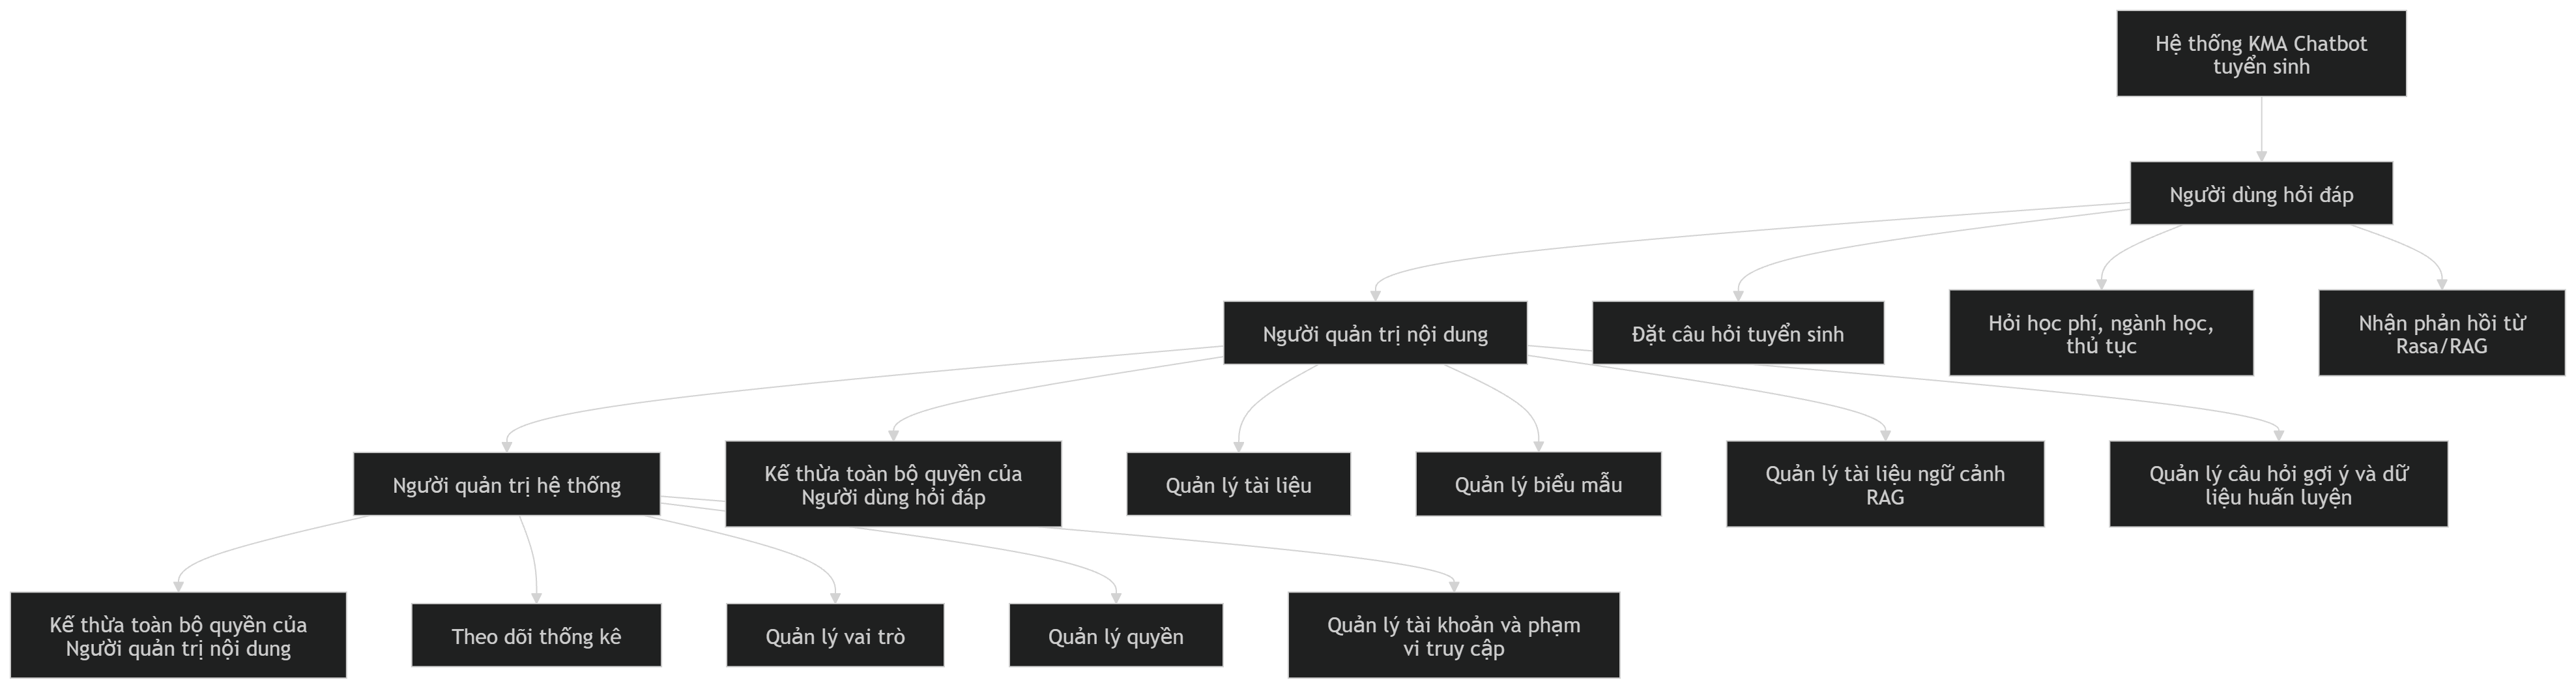
\includegraphics[width=0.8\textwidth]{content/source/User group diagram of the system.png}
    \caption{Sơ đồ các nhóm đối tượng sử dụng hệ thống}
    \label{fig:user_groups_overview}
\end{figure}

Người dùng hỏi đáp là nhóm sử dụng phổ biến nhất, tập trung vào việc đặt câu hỏi bằng ngôn ngữ tự nhiên để tra cứu thông tin tuyển sinh, ngành học, học phí, điểm chuẩn, thủ tục hoặc các biểu mẫu liên quan. Nhóm này chỉ tương tác ở mức khai thác thông tin nên không có quyền thay đổi dữ liệu, đồng thời phụ thuộc trực tiếp vào chất lượng tri thức mà hệ thống Rasa và RAG cung cấp.

Người quản trị nội dung giữ vai trò duy trì độ chính xác của kho tri thức. Họ phụ trách cập nhật tài liệu tuyển sinh, biểu mẫu, tài liệu ngữ cảnh cho RAG, câu hỏi gợi ý và một phần dữ liệu huấn luyện để chatbot luôn phản hồi đúng với quy định hiện hành. Trong khi đó, người quản trị hệ thống chịu trách nhiệm ở phạm vi rộng hơn, bao gồm quản lý tài khoản, vai trò, quyền truy cập, thống kê hoạt động và giám sát vận hành toàn bộ hệ thống.

Như vậy, sự khác biệt cốt lõi giữa ba nhóm người dùng nằm ở phạm vi thao tác: người dùng hỏi đáp chỉ khai thác thông tin, người quản trị nội dung được phép cập nhật nguồn dữ liệu phục vụ chatbot, còn người quản trị hệ thống kiểm soát hạ tầng quyền hạn và hoạt động chung. Cách phân tách này giúp hệ thống vừa hỗ trợ tư vấn thuận tiện cho người dùng cuối, vừa bảo đảm dữ liệu và vận hành được kiểm soát theo đúng trách nhiệm.

\begin{table}[H]
    \centering
    \caption{So sánh phạm vi sử dụng giữa các nhóm người dùng}
    \small
    \begin{tabularx}{\textwidth}{|p{3cm}|p{3cm}|X|p{2.5cm}|}
        \hline
        \textbf{Nhóm người dùng} & \textbf{Mục tiêu sử dụng} & \textbf{Phạm vi chức năng chính} & \textbf{Quyền thay đổi dữ liệu} \\ \hline
        Người dùng hỏi đáp & Tra cứu và nhận tư vấn tuyển sinh & Đặt câu hỏi cho chatbot, tra cứu thông tin ngành học, học phí, điểm chuẩn, thủ tục, văn bản & Không \\ \hline
        Người quản trị nội dung & Duy trì nguồn tri thức phục vụ chatbot & Quản lý tài liệu, biểu mẫu, tài liệu RAG, câu hỏi gợi ý và một phần dữ liệu huấn luyện & Có, trong phạm vi nội dung \\ \hline
        Người quản trị hệ thống & Quản lý vận hành và phân quyền & Quản lý tài khoản, vai trò, quyền truy cập, thống kê và kiểm soát hoạt động hệ thống & Có, trong phạm vi hệ thống \\ \hline
    \end{tabularx}
\end{table}
